% Figures exported by eval/build_thesis_assets.py (2026-11-13). Needs graphicx. Captions from figures_thesis/captions/*.md.

\begin{figure}[p]
\centering
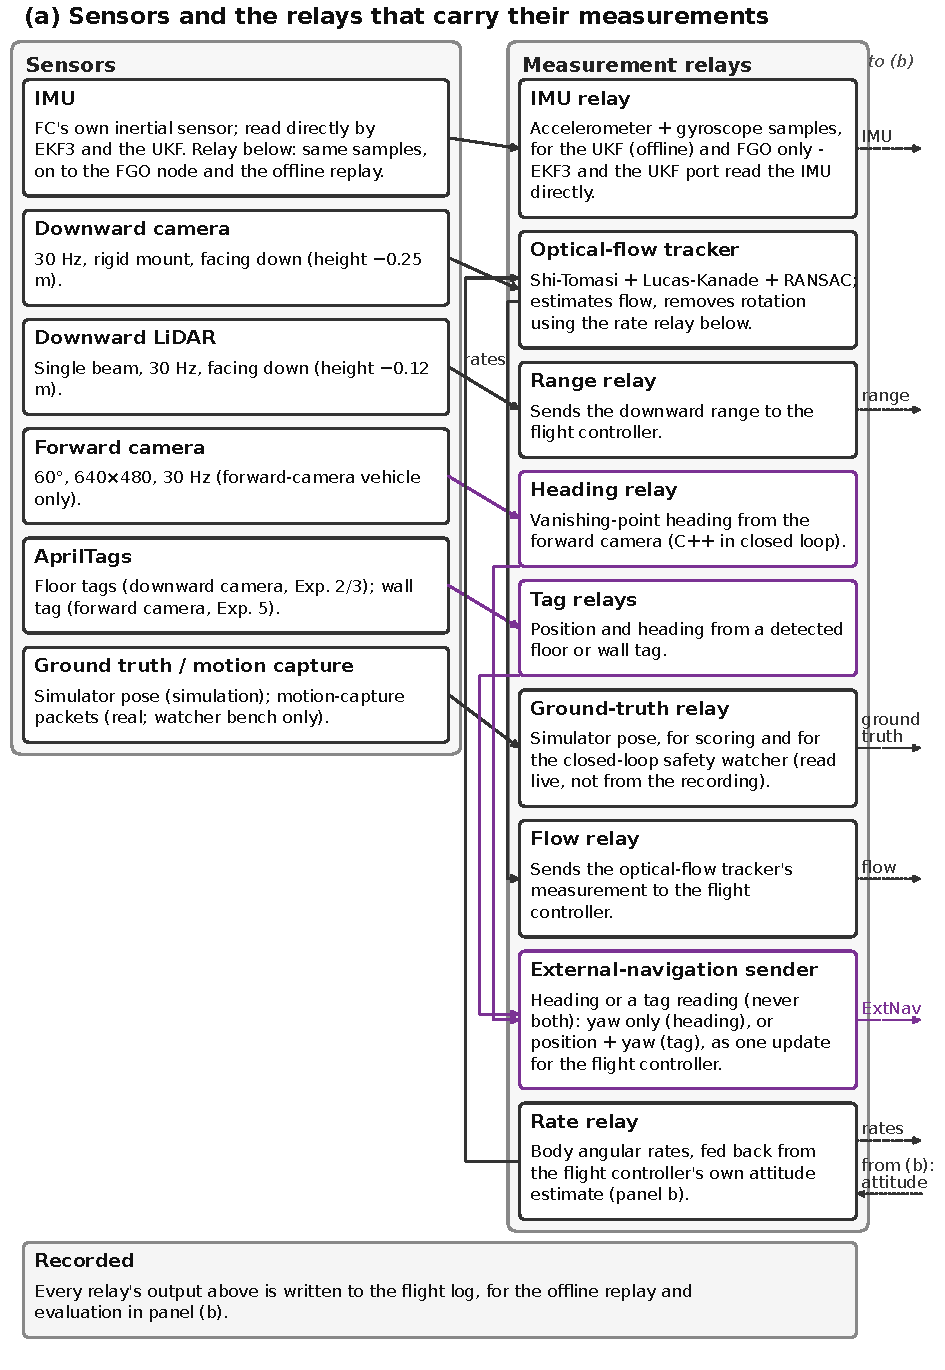
\includegraphics[width=\linewidth]{figures/fig_3-1a.pdf}
\caption[System architecture: sensors, bridges, the three estimators and where each one runs.]{System architecture: sensors, bridges, the three estimators and where each one runs. Panel (a) shows the sensors and the relays that carry their measurements to the flight controller and to the recorded data used offline. Panel (b) shows the flight controller, where each of the three estimators runs, outlined in its own colour (EKF3 blue, UKF green, FGO orange), alongside the safety watchers and the offline replay and evaluation. Verdicts: Table A.4, none (descriptive).}
\label{fig:3-1}
\end{figure}
\begin{figure}[p]
\centering
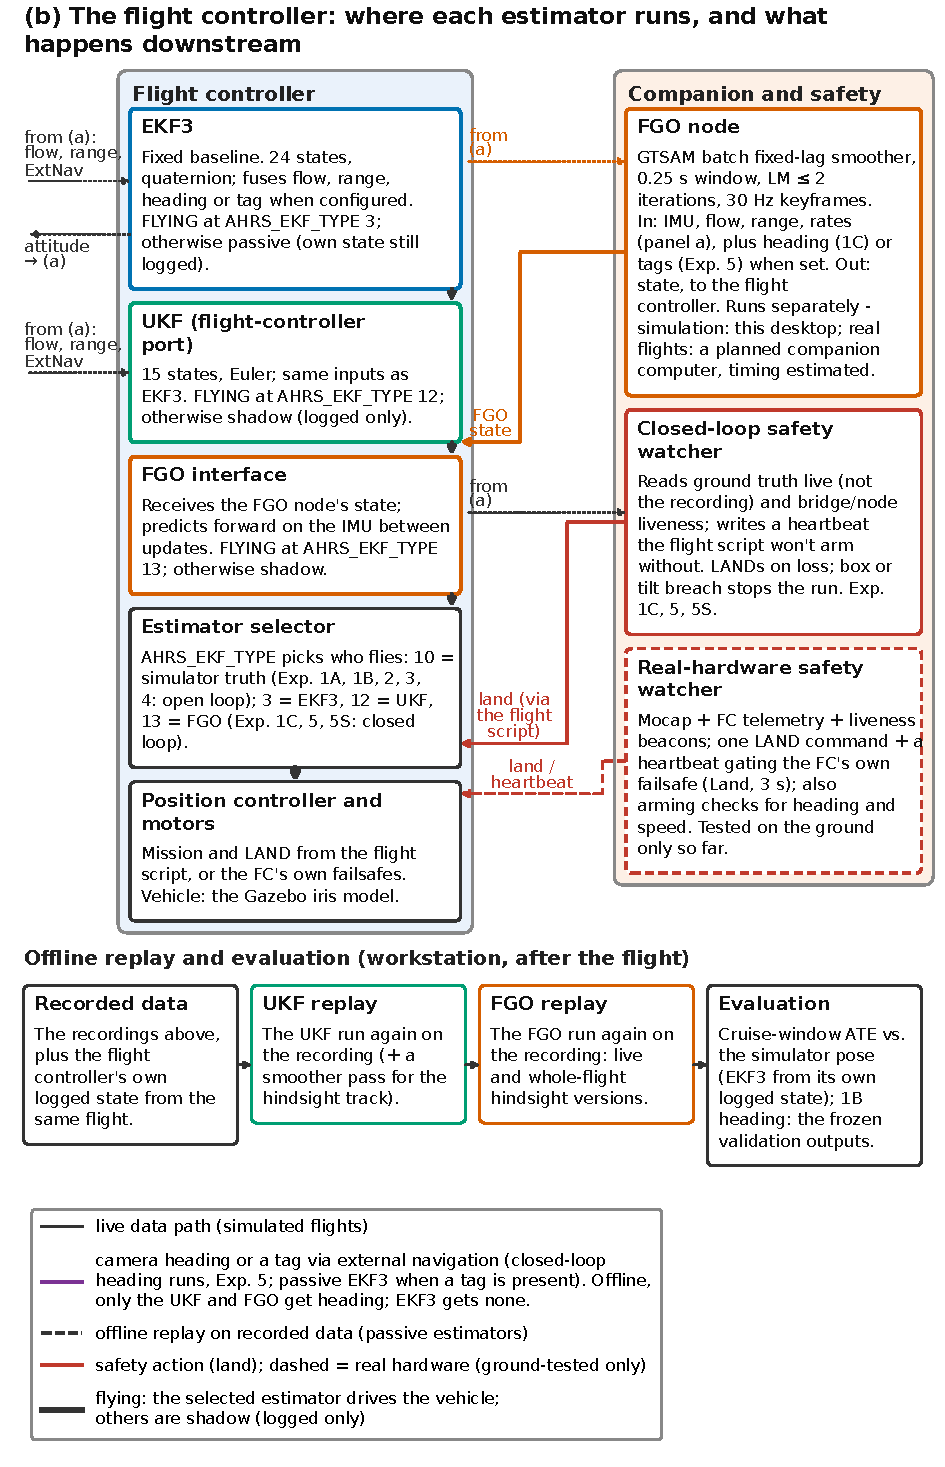
\includegraphics[width=\linewidth]{figures/fig_3-1b.pdf}
\caption*{Figure 3.1 (continued): panel (b).}
\end{figure}

\begin{figure}[htbp]
\centering
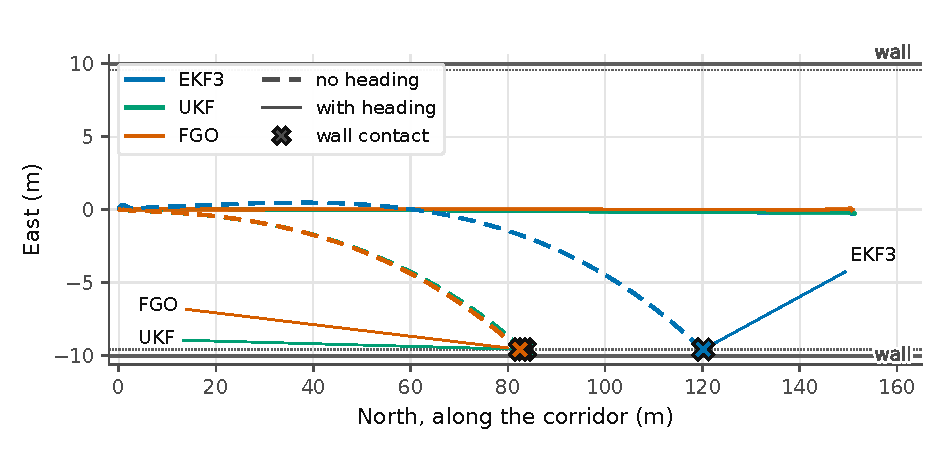
\includegraphics[width=\linewidth]{figures/fig_4-1.pdf}
\caption[The camera heading stops the sideways drift: without it every estimator flies into the west wall.]{The camera heading stops the sideways drift: without it every estimator flies into the west wall. Each estimator's flown path through the textured corridor, top-down, with the lateral (East) axis stretched 3.0x and walls at x = $\pm$10 m; the dotted line marks the 9.58 m contact threshold. Colour shows the flying estimator: dashed lines are one no-heading flight each, run to wall contact (marked by X); solid lines are three with-heading flights per estimator, which overlap near the centreline at this scale. Heading-error detail is in Table 4.3 and Figure 4.1b (provisional). Verdicts: Table A.4, rows H1.8 n = 3 EKF3, half real-time (RTF 0.5); H1.8 n = 3 UKF, half real-time (final port, abb0357d); H1.8 n = 3 FGO, half real-time (corrected priors, 4c07374b/HEAD); H1.9 EKF3; H1.9 UKF (final UKF port, half real-time); H1.9 FGO (corrected priors, 4c07374b/HEAD, half real-time).}
\label{fig:4-1}
\end{figure}

\begin{figure}[htbp]
\centering
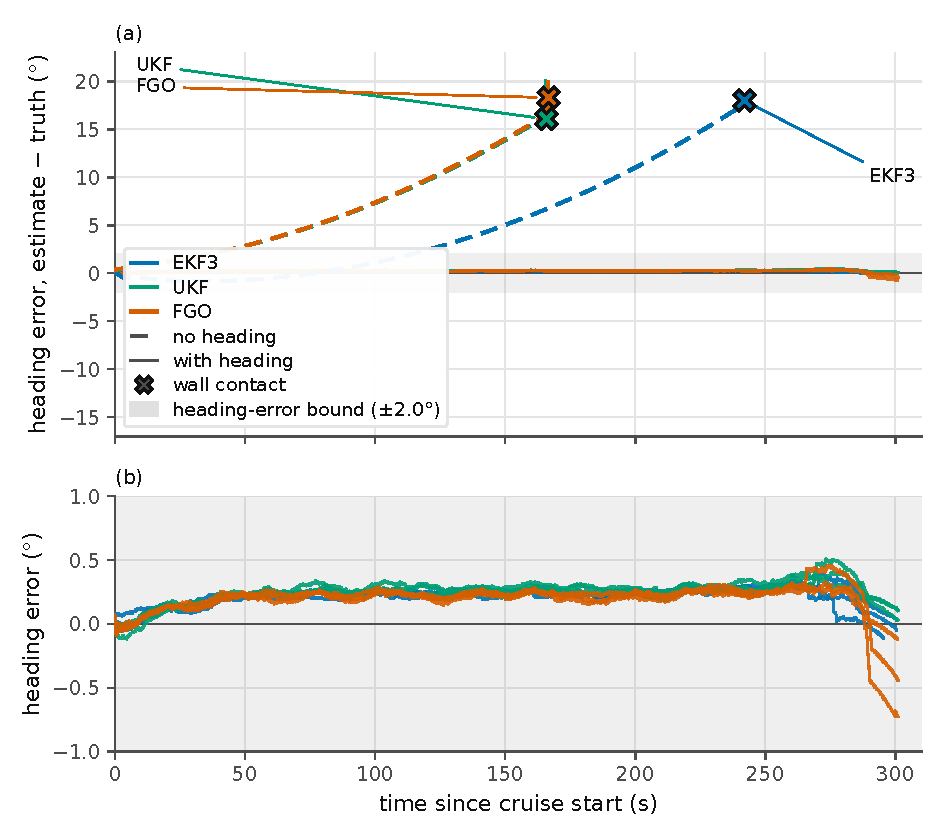
\includegraphics[width=\linewidth]{figures/fig_4-1b.pdf}
\caption[Without a heading source the heading error grows until the wall; with the camera heading it stays near zero.]{Without a heading source the heading error grows until the wall; with the camera heading it stays near zero. Heading error of the flying estimator (current yaw minus the simulator's true yaw) against time since cruise start, on the same closed-loop flights as Figure 4.1. Colour shows the flying estimator; dashed lines are one no-heading flight each, ending at wall contact at +242.1 s (EKF3), +165.9 s (UKF) and +166.7 s (FGO); solid lines are three with-heading flights per estimator. With the camera heading, in panel (a) all 9 flights' lines sit on zero against the grey $\pm$2.0\textdegree{} heading-error band; panel (b) shows the same with-heading flights alone, on a linear $\pm$1\textdegree{} scale. Verdicts: Table A.4, rows H1.8 n = 3 EKF3, half real-time (RTF 0.5); H1.8 n = 3 UKF, half real-time (final port, abb0357d); H1.8 n = 3 FGO, half real-time (corrected priors, 4c07374b/HEAD); H1.9 EKF3; H1.9 UKF (final UKF port, half real-time); H1.9 FGO (corrected priors, 4c07374b/HEAD, half real-time).}
\label{fig:4-1b}
\end{figure}

\begin{figure}[htbp]
\centering
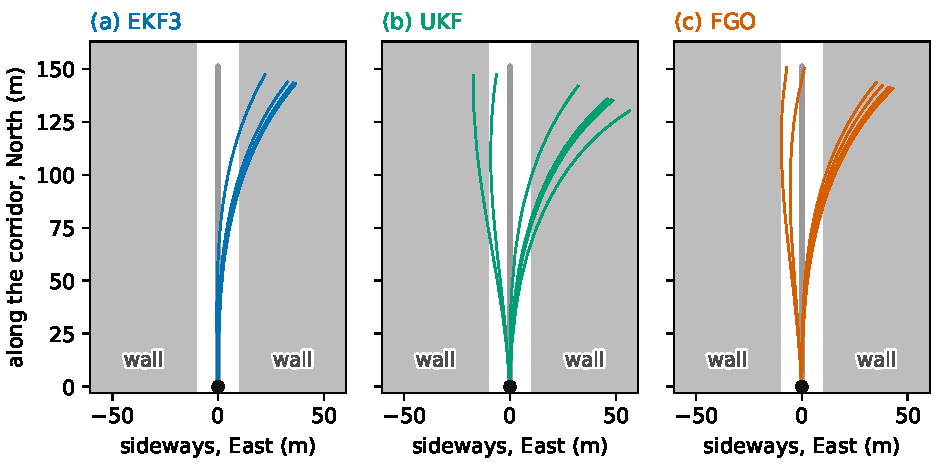
\includegraphics[width=\linewidth]{figures/fig_4-1d.pdf}
\caption[Without a heading source, every one of the 9 flights drifts sideways off the true path.]{Without a heading source, every one of the 9 flights drifts sideways off the true path. Raw (unaligned) top-down paths for all 9 flights of the standard-sensor dataset, textured floor, no heading source: one panel per estimator, EKF3 (blue), UKF (green) and FGO (orange), truth in grey, each estimate drawn in its own navigation frame with its origin at take-off (black dot). The shaded bands are the corridor walls; East and North are drawn at equal scale (1.0$\times$). Fitted and raw values are in Table 4.4 (provisional). Verdicts: Table A.4, rows H1.1.}
\label{fig:4-1d}
\end{figure}

\begin{figure}[htbp]
\centering
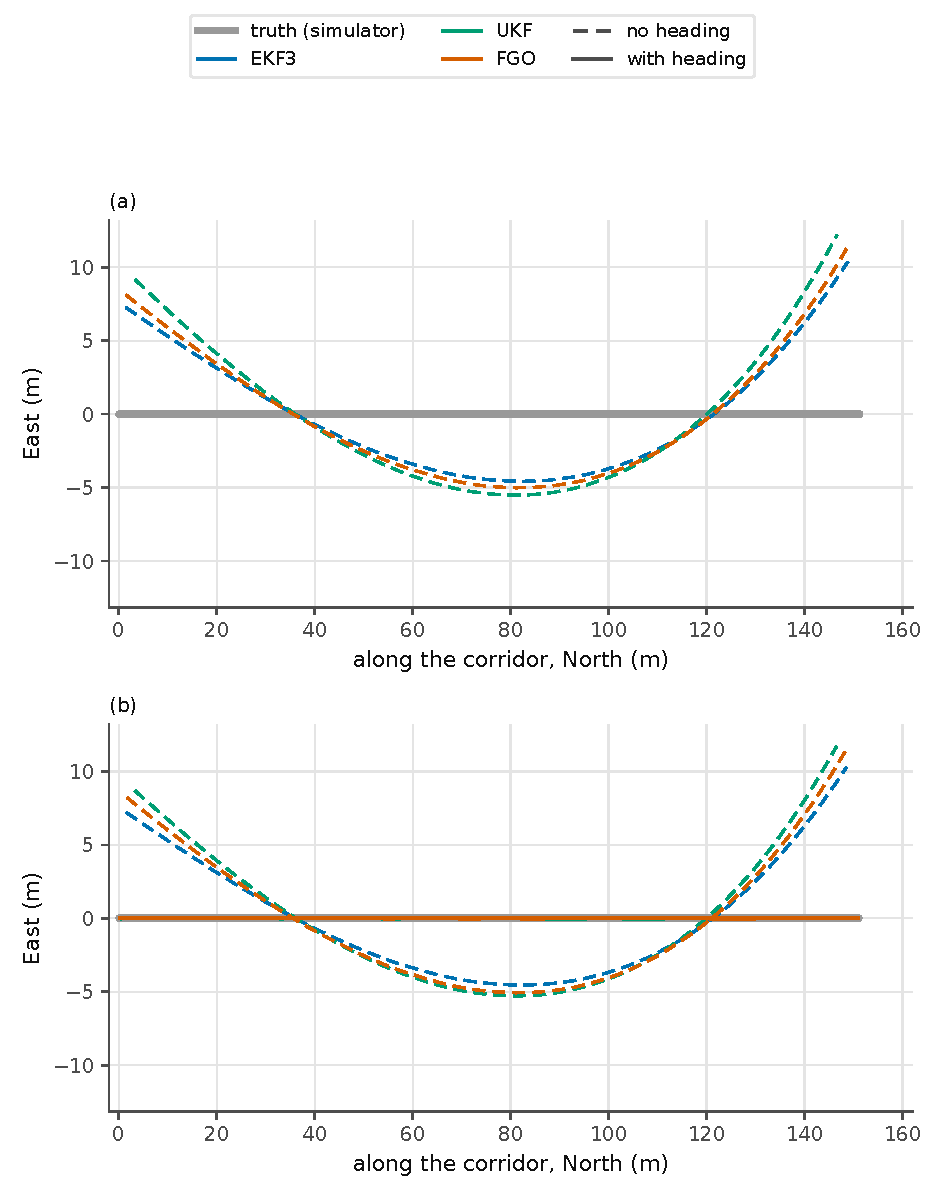
\includegraphics[width=\linewidth]{figures/fig_4-2.pdf}
\caption[True and estimated paths, top-down: with the camera heading the UKF and FGO paths lie on the true path.]{True and estimated paths, top-down: with the camera heading the UKF and FGO paths lie on the true path. True and estimated top-down paths for EKF3 (blue), UKF (green) and FGO (orange) against truth (grey), each path aligned to its own ground-truth file by a best-fit rotation and shift (no scale) over the cruise window. Panel (a) is flight 3 of the standard-sensor dataset, no heading source (dashed); panel (b) is flight 3 of the textured-wall camera dataset, shown both without heading (dashed) and with the camera heading (solid, UKF and FGO only). The East axis is stretched 3.0$\times$ relative to North. Verdicts: Table A.4, none (descriptive).}
\label{fig:4-2}
\end{figure}

\begin{figure}[htbp]
\centering
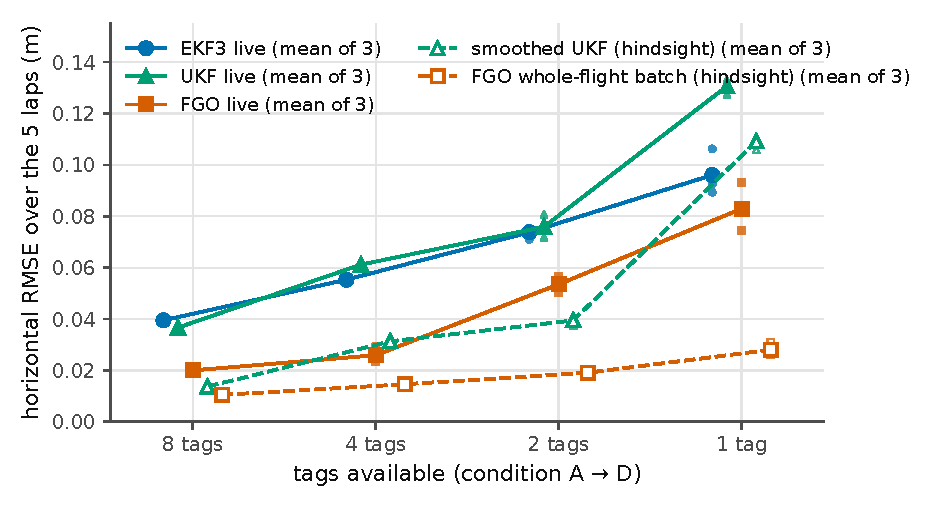
\includegraphics[width=\linewidth]{figures/fig_5-1.pdf}
\caption[Fewer tags, larger live errors; the FGO's hindsight batch stays at 0.01--0.03 m.]{Fewer tags, larger live errors; the FGO's hindsight batch stays at 0.01--0.03 m. Experiment 2 (known tags): horizontal RMSE in the world frame against which tags are available (condition A all 8, B the four corners, C two diagonal, D one tag). Colour and marker show the estimator; solid filled lines are live, dashed open lines are hindsight (the FGO whole-flight batch and the smoothed UKF); small marks show each of three flights, with a line through their mean. Live errors grow as tags thin out from condition A to D, while the FGO's hindsight batch stays flat across all four conditions. Verdicts: Table A.4, rows H2.1; H2.2; H2.3; H2.4.}
\label{fig:5-1}
\end{figure}

\begin{figure}[htbp]
\centering
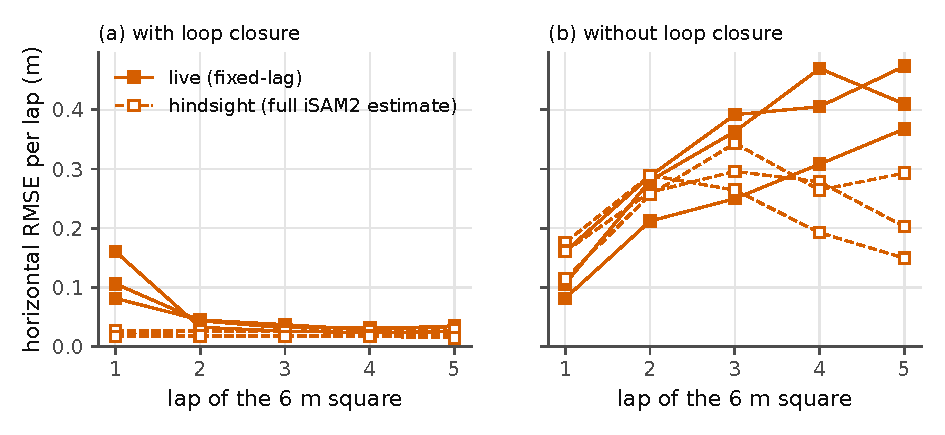
\includegraphics[width=\linewidth]{figures/fig_5-2.pdf}
\caption[Re-identifying tags at unknown positions keeps the FGO's error flat; without it the error grows 2.9 to 4.5 times over five laps.]{Re-identifying tags at unknown positions keeps the FGO's error flat; without it the error grows 2.9 to 4.5 times over five laps. Experiment 3 (loop closure): the keyframe FGO with AprilTags at unknown positions, each tag treated as a landmark, flights 1 to 3, horizontal RMSE per 6 m lap in the first tag's frame, on one shared linear axis; live is solid and filled, hindsight is dashed and open. Left: with loop closure the live error falls after lap 1; right: without re-identification it grows over five laps. The thesis's EKF3 and UKF, as configured, have no landmark states, so only the FGO shows loop closure here; in extension tests with 4 tags and with 2 tags, the FGO's loop closure also bounded live drift in 3/3 flights in each, but with 1\% wrong tag IDs its live error with loop closure was below the no-loop-closure error on the same flight in 0/9 runs (6 of 9 runs diverged). Verdicts: Table A.4, rows V3; H3.1; H3.2; H3.3; H3.4; Extension E2 H-E2.1; Extension E3 H-E3.1; Extension E5 H-E5.1; Extension E5 S-E5.5.}
\label{fig:5-2}
\end{figure}

\begin{figure}[htbp]
\centering
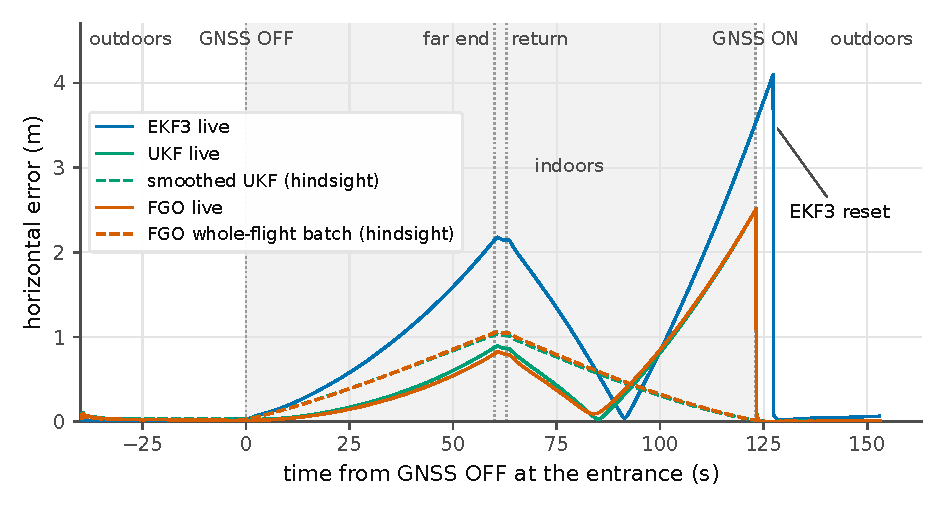
\includegraphics[width=\linewidth]{figures/fig_5-3.pdf}
\caption[Indoors without GNSS the live tracks drift and EKF3 jumps 4.1 m on return, about 4.3 s after GNSS returns (the switching script's delay); hindsight keeps the error near 1 m.]{Indoors without GNSS the live tracks drift and EKF3 jumps 4.1 m on return, about 4.3 s after GNSS returns (the switching script's delay); hindsight keeps the error near 1 m. Experiment 4 (outdoor-indoor), flight 1: horizontal error against time in the world frame, as the vehicle flies outdoors, through a GNSS-denied indoor section, and back outdoors. Route events (dotted lines): GNSS OFF at the entrance (0 s); the far end reached at about 60 s; the return starting at 63 s; GNSS ON at 123 s. Solid lines are live, dashed lines are hindsight; EKF3 resets to GNSS on return with a 4.10 m jump, about 4.3 s after GNSS returns once the simulation's GNSS switching script moves EKF3 off its indoor source set, with no such delay for the UKF or FGO. Verdicts: Table A.4, rows H4.1; H4.2; H4.3.}
\label{fig:5-3}
\end{figure}
